\section{Model-Based RL}\label{sec:model-based}
In the previous section Actor-Critic methods were implemented on both the CartPole and Catch environments. The inclusion of a inductive bias exploiting the symmetry of an MDP lead to improvements in the sample efficiency of learning an expert policy, while maintaining robustness to initialization conditions.

While this methodology was effective in improving the learning dynamics of the agent, the hard requirement for the symmetry of the environment is a strong constraint.

In the case of a model-based agent, that performs planning and acting phases, the agent requires both a world model $T_\phi : \mathcal{S} \times \mathcal{A}\rightarrow \mathcal{S}, R_\psi :\mathcal{S} \times \mathcal{A}\rightarrow \mathbb{R}, $ and a policy or value model, $\pi_\theta(s)$.

In the case where the transition dynamics of the MDP are group structured, or approximately group structured, this report proposes the use of an Equivariant world model. With a world model that has inductive biases that are designed to aid in learning the MDP's transition dynamics, the world model may be learned more efficiently and accurately from fewer samples from the environment, improving the effectiveness of planning for the agent. Additionally, because the policy that is learnt is not required to be equivariant, the agent may also still perform well in situations where the symmetry is not exact. The initial experementation uses a simple hybrid model-based algorithm, that has both model-based and model-free components Dyna.

Dyna alternates between planning and acting phases, where the agent's policy is learned from experience in the MDP, an Acting phase. Then the agent learn's a world model and then performs a planning phase. Planning is where the agent simulates trajectories, with it's learned world model and updates its policy from the simulated trajectories.


\subsection{Constructing Transition Models}
Before using a full model-free algorithm, where the model is learned online, during the training. A simplified algorithm, Supervised-Dyna, is tested that uses off-line trained world models. The process for this is outlined below:
\begin{algorithm}
	\caption{Supervised-Dyna}
	\begin{algorithmic}
		\State Initialize $T_\phi$
		\State Sample transition tuples from a policy $\pi \sim (s, a, s')$ on MDP $\mathcal{M}$.
		\Comment {Here $\pi$ is a random/ expert policy}
		\State Form Dataset $\mathcal{D}$ from sampled transition tuples.
		\For {Num Epochs}
		\State $\phi' \leftarrow $Minimise $L(\phi , \mathcal{D})$.
		\EndFor
		\For {Num Dyna Iterations}
		\For {Num Acting Updates}
		\State Sample transition tuples from policy $\pi_\theta \sim (s, a, s')$ on $\mathcal{M}$
		\State Train agent $\pi_\theta$ from direct samples.
		\EndFor
		\For{Num Planning Updates}
		\State Sample transition tuples from policy $\pi_\theta \sim (s, a, s')$ on $T_\phi$.
		\State Train agent $\pi_\theta$ from planned samples.
		\EndFor
		\EndFor
	\end{algorithmic}
\end{algorithm}

Using off-line trained world models has benefits as an intermediate step. Firstly, the world model is stationary throughout the agent training process and can be easily investigated. Secondly, the model can be trained with ample data. This is in contrast to full Dyna where, the length of the planning and acting phases must be tuned as a hyper parameter, and the convergence of the models must be tuned.


\subsection{Proximal Pooling Motivation}

To produce equivariant world models, there are additional challenges beyond that of just implementing a G-CNN which permutes its outputs dependent on the input transformation. In contrast to an equivariant actor where simply permuting the logits of a distribution suffices to have equivariant behaviour \ref{symmetrizer}. When building an equivariant world model with a G-CNN, the output of the network predicts the next state and a number of nonsense next states.

To illustrate what the final layer output in the G-CNN is doing, consider the same setup as the Actor-Critic networks, where there is a hidden representation that's responses get permuted depending on the application of a group structured transformation on the input:

\begin{equation}
	f(s , a) = \begin{pmatrix}
		g(s, a)                                     \\
		g(\ell_1^\mathcal{S}s,\ell^\mathcal{A}_1a)  \\
		g(\ell^\mathcal{S}_2s, \ell^\mathcal{A}_2a) \\
		\vdots                                      \\
		g(\ell_{|G|}^\mathcal{S}s, \ell^\mathcal{A}_{|G|}a),
	\end{pmatrix}
\end{equation}
and when a transformation is applied to the input these responses, $g$ are permuted,
\begin{equation}\label{eq:tm_gcnn}
	f(\ell_i^\mathcal{S}s, \ell_i^\mathcal{A}a) = \mat{P}_i f(s, a).
\end{equation}
Because the permutations are defined by the group, these are the same permutations as in Eq.\ref{eq:gs_perm}. However here each response $g: \mathcal{S} \times \mathcal{A} \rightarrow \mathcal{S}$. In order to get a transition function there must be a method to pool over the responses.

\subsection{Group Action Transformation}
When the network $f$ performs a forward pass and outputs the vector of responses, Eq.\ref{eq:tm_gcnn}, the equivariance in the response is mapping group actions on a state space to a permutation of responses that are all the same shape as the state. This is not the equivariance constraint that is required for a transition model, which is,
\begin{equation}
	T(\ell_i^\mathcal{S}s, \ell_i^\mathcal{A}a) = \ell_i^\mathcal{S}T(s, a).
\end{equation}
The first step in achieving this is to apply a group action to each row of the response of $f$. This is the Action Transformation operation denoted as $\mat{\mathcal{T}}$, where,
\begin{equation}
	\mat{\mathcal{T}}f(s,a) = \begin{pmatrix}
		g(s, a)                                                          \\
		\ell_{-1}^\mathcal{S}g(\ell_1^\mathcal{S}s,\ell^\mathcal{A}_1a)  \\
		\ell_{-2}^\mathcal{S}g(\ell^\mathcal{S}_2s, \ell^\mathcal{A}_2a) \\
		\vdots                                                           \\
		\ell_{-|G|}^\mathcal{S}g(\ell_{|G|}^\mathcal{S}s, \ell^\mathcal{A}_{|G|}a)
	\end{pmatrix}.
\end{equation}
Due to group closure, this gets us quite close to equivariance! For example consider some group element, which is the inverse of $i$ acting on the input,

\begin{equation}\label{eq:g-cnn}
	\mat{\mathcal{T}}f(\ell_{-i}^\mathcal{S}s,\ell_{-i}^\mathcal{A}a) = \begin{pmatrix}
		g(\ell_{-i}^\mathcal{S}s,\ell_{-i}^\mathcal{A}a)                 \\
		\ell_{-1}^\mathcal{S}g(\ell_j^\mathcal{S}s,\ell^\mathcal{A}_ja)  \\
		\ell_{-2}^\mathcal{S}g(\ell^\mathcal{S}_ks, \ell^\mathcal{A}_ka) \\
		\vdots                                                           \\
		\ell_{-i}^\mathcal{S}g(s, a)                                     \\
		\vdots                                                           \\
		\ell_{-|G|}^\mathcal{S}g(\ell_{|G|}^\mathcal{S}s, \ell^\mathcal{A}_{|G|}a)
	\end{pmatrix}.
\end{equation}
Then to achieve equivariance, the correct row must be selected. This would be straightforward if the group action on the input was known, but in general it is not. However, in many cases, in a transition model, the output is closer to the input than any of the other states! With this proximity intuition a pooling method is introduced to gain approximate equivariance with the transition models. This vector of next states, is referred to as transition images.

When using Conv-nets or other G-CNNs for classification or other image processing tasks, a reduction pooling such as mean or max is used over the different groups. Both of these pooling types result in an invariant network, where, if one pools over the group, takes a mean or a max over the group dimension of $f$, because the transformation only applies a permutation along this axis there is no change in the output if the group dimension is permuted,
\begin{equation}
	\max_\text{axis G} \mat{P}_i f(s, a) = \max_\text{axis G} \mat{P}_j f(s, a), \forall i, j.
\end{equation}
Here the group axis, axis G, is the leading dimension in $f$ if $f: \mathcal{S} \times \mathcal{A} \rightarrow \mathbb{R}^{|G| \times \mathcal{S}}$. This invariance is not helpful in our case and so an alternative technique of pooling over possible next states is proposed.


\subsection{Proximal Pooling Layers}
As a forward, this method does not guarantee equivariance to the input transformation. However, empirically it is effective.
The proximal pooling layer$\mathcal{P}$, takes a distance metric, $d(s, s')$, and selects the transition image, which has the minimum distance metric, as such the full approximately equivariant network is;
\begin{equation}
	\mathcal{P}\mathcal{T}f(s, a)  =\arg \min_\text{axis G} d \left (s,  \begin{pmatrix}
			g(s, a)                                                          \\
			\ell_{-1}^\mathcal{S}g(\ell_j^\mathcal{S}s,\ell^\mathcal{A}_ja)  \\
			\ell_{-2}^\mathcal{S}g(\ell^\mathcal{S}_ks, \ell^\mathcal{A}_ka) \\
			\vdots                                                           \\
			\ell_{-|G|}^\mathcal{S}g(\ell_{|G|}^\mathcal{S}s, \ell^\mathcal{A}_{|G|}a)
		\end{pmatrix}
	\right ).
\end{equation}
The $\arg \min_\text{axis G}$, returns the state image, which is closest to the original state, if the network predictions are better than random with respect to the distance metric.

Empirically across 10,000 randomly sampled CartPole states, the network, $T(s, a)= \mathcal{P}\mathcal{T}f(s,a)$, is fully equivariant, when untrained. When trained, it is equivariant across the same sample, and also achieves better validation MSE than the non equivariant model, when trained on transitions from the same data.

This is not the case for the Catch network. Catch has $675$ state action pairs, and the transition model when untrained achieves $98.3 \pm 0.6\%$ equivariance, across all these state action pairs. The standard error is quoted over 1000 random seed parameter initializations. The performance of the transition models is investigated in more depth, in sections\ref{something,something}.

When trained, the Catch model is able to achieve validation accuracy of 1. As such, the lack of perfect equivariance, may not be an issue in some scenarios. Small discrete spaces, with a high degree of symmetry are the worst in terms of a lack of equivariant predictions, as the expected distance between any two states decreases. Additionally, for MDPs where no sensible distance metric can be constructed this method will fail.
\begin{proposition}
	Given some distance metric between two states $d(s, s')$ and a G-CNN transition model of the form Eq.\ref{eq:g-cnn}. If at some time $t$ a state transition from $s_t$ to $s_{t+1}$ takes place. And the MDP has a group structured discrete symmetry, if the state space obeys,
	\begin{equation}
		d(s_t, s_{t+1}) < \mathbb{E}_{s'\sim \mu}[d(s_t, s')], \forall i, s_t.
	\end{equation}
	Where $\mu$ is the steady state distribution. Then, a proximal pooling layer can be used to make the G-CNNs' forward pass approximately equivariant.
\end{proposition}
As motivation for why this is, when the G-CNN performs a forward pass, one of the multiple outputs of $\mathcal{T} f(\ell_i^\mathcal{S}s,\ell_i^\mathcal{A} a)$, are empirically not correlated to the other group members, for all parts of the state effected by the transformations.
\begin{figure}[h!]
	\centering
	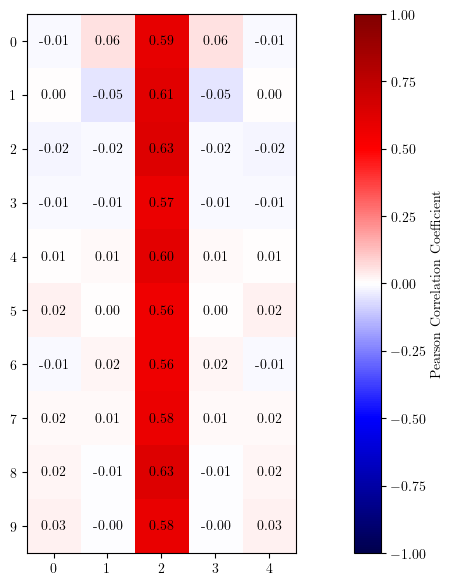
\includegraphics[width = 0.5\textwidth]{Figures/logits_correlation.png}
	\caption{Pearson Correlation }
	\label{fig:logits_correlation}

\end{figure}

\subsection{CartPole}
A CartPole transition model is a functional approximation to a deterministic Non linear system. In CartPole the transitions between different states in CartPole are governed by the PDEs:
\begin{equation}
\ddot{\theta} = \frac{g \sin \theta + \cos\theta \left({\frac{-F - m_p l \dot{\theta}^2 \sin(\theta)}{m_c + m_p}} \right )}{l\left ( \frac{4}{3} - \frac{m_p \cos^2 \theta}{m_c + m_p}\right)},
\end {equation}

\begin{equation}
	\ddot{x} = \frac{ F + m_p l (\dot{\theta}^2 \sin \theta - \ddot{\theta} \cos \theta)}{m_c + m_p}.
\end{equation}
Here $g$ is the acceleration due to gravity and is positive, $\theta$ is the angle between the pole and vertical, with the pole length $l$. $F$ is the action force, where the positive direction is right. The masses of the cart and the pole are $m_c, m_p$, respectively. Finally $\dot{}$, indicates a derivative with respect to time.

These PDEs have no closed solution and their form is taken from \cite{florian2007correct} who provides slight corrections to the original dynamics in \cite{barto1983neuronlike}.

To learn this transition model, transitions are sampled from a policy on the MDP, and stored. This is then used as a dataset to perform supervised learning on. The Transition model, $T_\phi: \mathcal{S} \times \mathcal{A} \rightarrow \mathcal{S}$, predicts next states from a state action pair. A state is a vector s:
\begin{equation}
	s = \begin{pmatrix}
		x       \\
		\dot{x} \\
		\theta  \\
		\dot{\theta}
	\end{pmatrix}
\end{equation}
The loss function for the transition model is the average L2 distance between the predicted next state, and the true next state across a batch of samples.
\begin{equation}
	L(\phi) = \frac{1}{N}\sum^N_{(s, a, s')_i \sim \mathcal \tau} ||T(s, a) - s'||_2
\end{equation}
Here $\tau = \{(s, a , s')_1^N\}$ is a batch of transition, of size $N$, sampled from the MDP, and $(s, a, s')$, is the state, action, next state tuple. Often a reward model is required to also make an MDP. For simplicity, the CartPole reward model is used, rather than learned. As such the transition gains a reward of $+1$, if $|\theta| < 12.5^o$, otherwise the episode terminates.

\subsubsection{Constructing Equivariant World Models}
Like in the previous section on \ref{sec:actor-critic}, the equivariant transition models are deep G-CNNs. In contrast to the previous section, these networks





